\documentclass{article}
\usepackage[utf8]{inputenc}
\usepackage{clrscode3e}
\usepackage[english]{babel}
\usepackage{blindtext}
 \usepackage{graphicx}
 \usepackage{hyperref}
 \hypersetup{
    colorlinks=true,
    linkcolor=blue,
    filecolor=magenta,      
    urlcolor=cyan,
}
\urlstyle{same}
\pagestyle{plain}
\begin{document}

\graphicspath{ {./images/} } 
\begin{titlepage}
 
   \begin{center}
   
       \vspace*{1cm}
       \Huge
       \textbf{Artificial Intelligence Homework} \vspace{1 cm}
       
       \textbf{Archer Problem Experimental Data}
            
       \vspace{1 cm}
      \LARGE
       \textbf{Buzdug\u{a} Ionu\c{t} Gabriel}\\
       Group CEN 2.1B\\
       Year 2\\
       Computer and Information Technology-English
       \vfill
            
      
            
       \vspace{0.8cm}
      
    
    \end{center}
  \end{titlepage}
\newpage


\section{Experimental data}
\Large
\vspace*{1cm}
\LARGE
\par In this section it is presented how the experimental values are generated
for our problem.
\par To test our problem we need to generate multiple data sets which are meaningful to our goals in finding how does our algorithm behave.
\par In order to achieve this we need to make use of the random input data generator located in the main file,which will be our data input reference.
\par The algorithm for the generator has been presented in the report under the Apllication outline when I presented how the main.py module works and what it contains.
\par In order to test our input data generator I ran the algorithm 10 times to get multiple data outputs which I will compare down below.
\par The output data consists of getting all the possible  arrangements for the archers and the walls visualised both in original form(a list of elements which tell the position of each archer on the board) and in form of a grid which helps both me and the reader to understand how the algorithm works.
\newpage

\subsection{Results and Conclusions}
\par In this section we will conduct a set of tests to observe how the algorithm behaves.
Here we have all 10 inputs tests made on different sizes of input data:small,medium,large.
\\In most of these tests I will show the first couple of arrangements found,and then the last ones together with the number of solutions found and the running time of the algorithm.
\Large
\begin{enumerate}
\item first test(small test size:grid size:5,walls placed on position:2)
\begin{figure}[h]
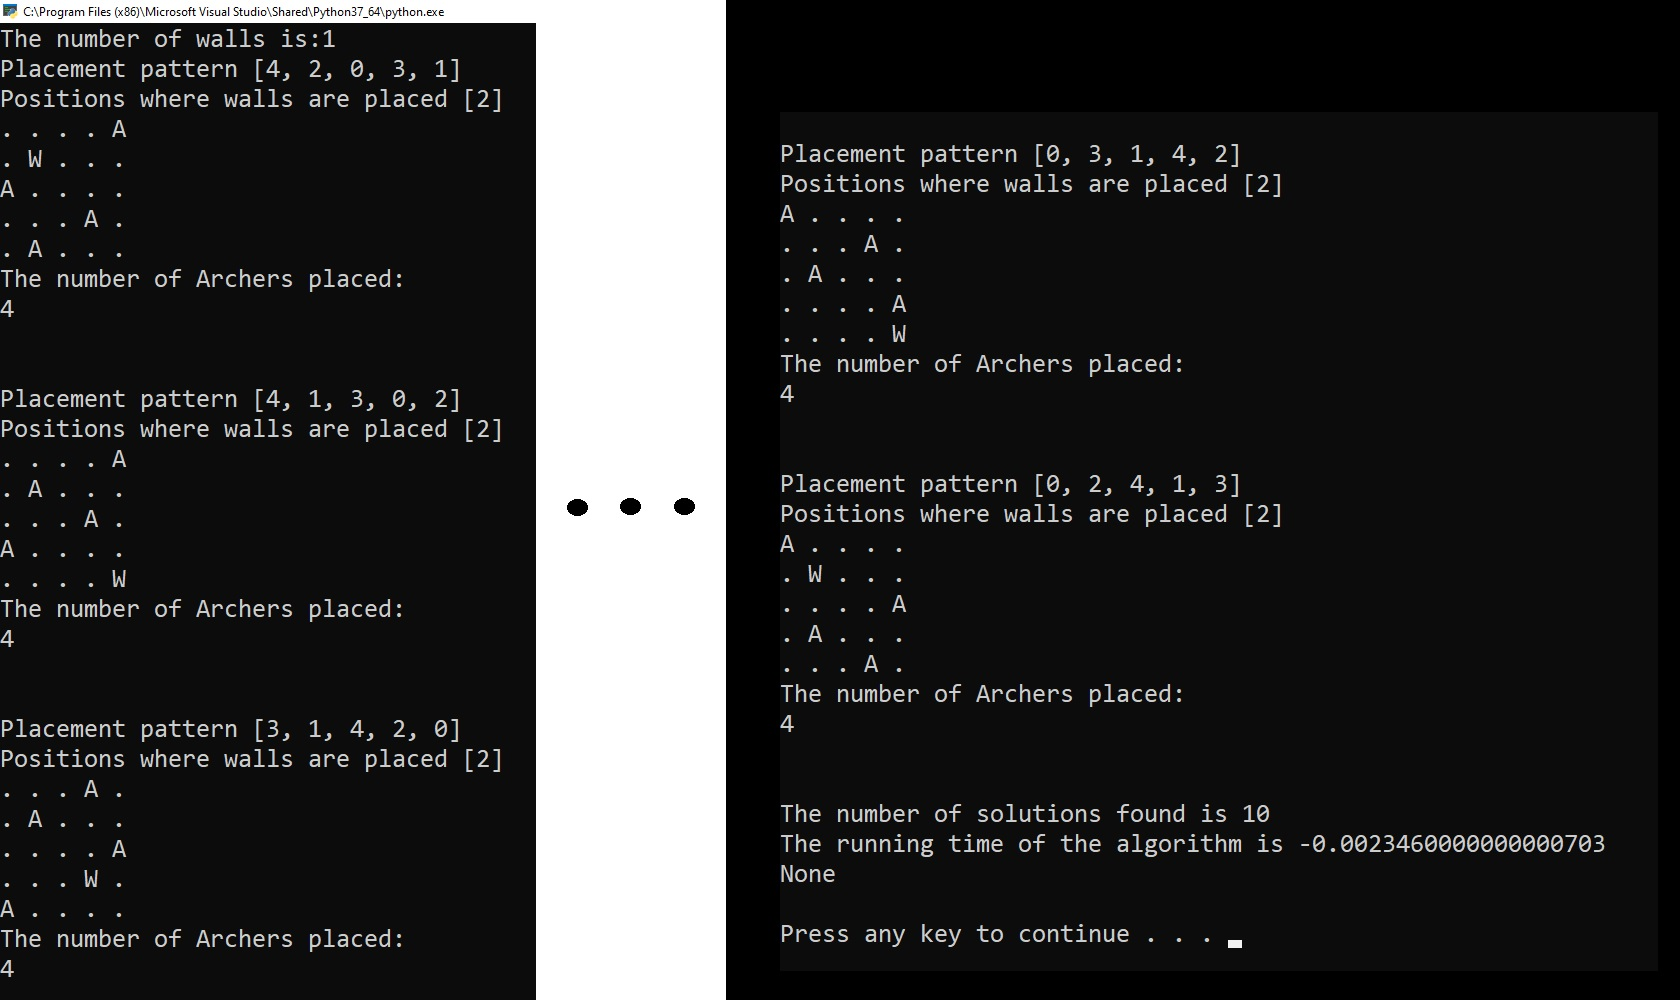
\includegraphics[width=12 cm, height=10cm]{test1}
\end{figure}
\newpage

\item second test(small test size,grid size:5,walls placed on positions:0,3,2)
\begin{figure}[h]
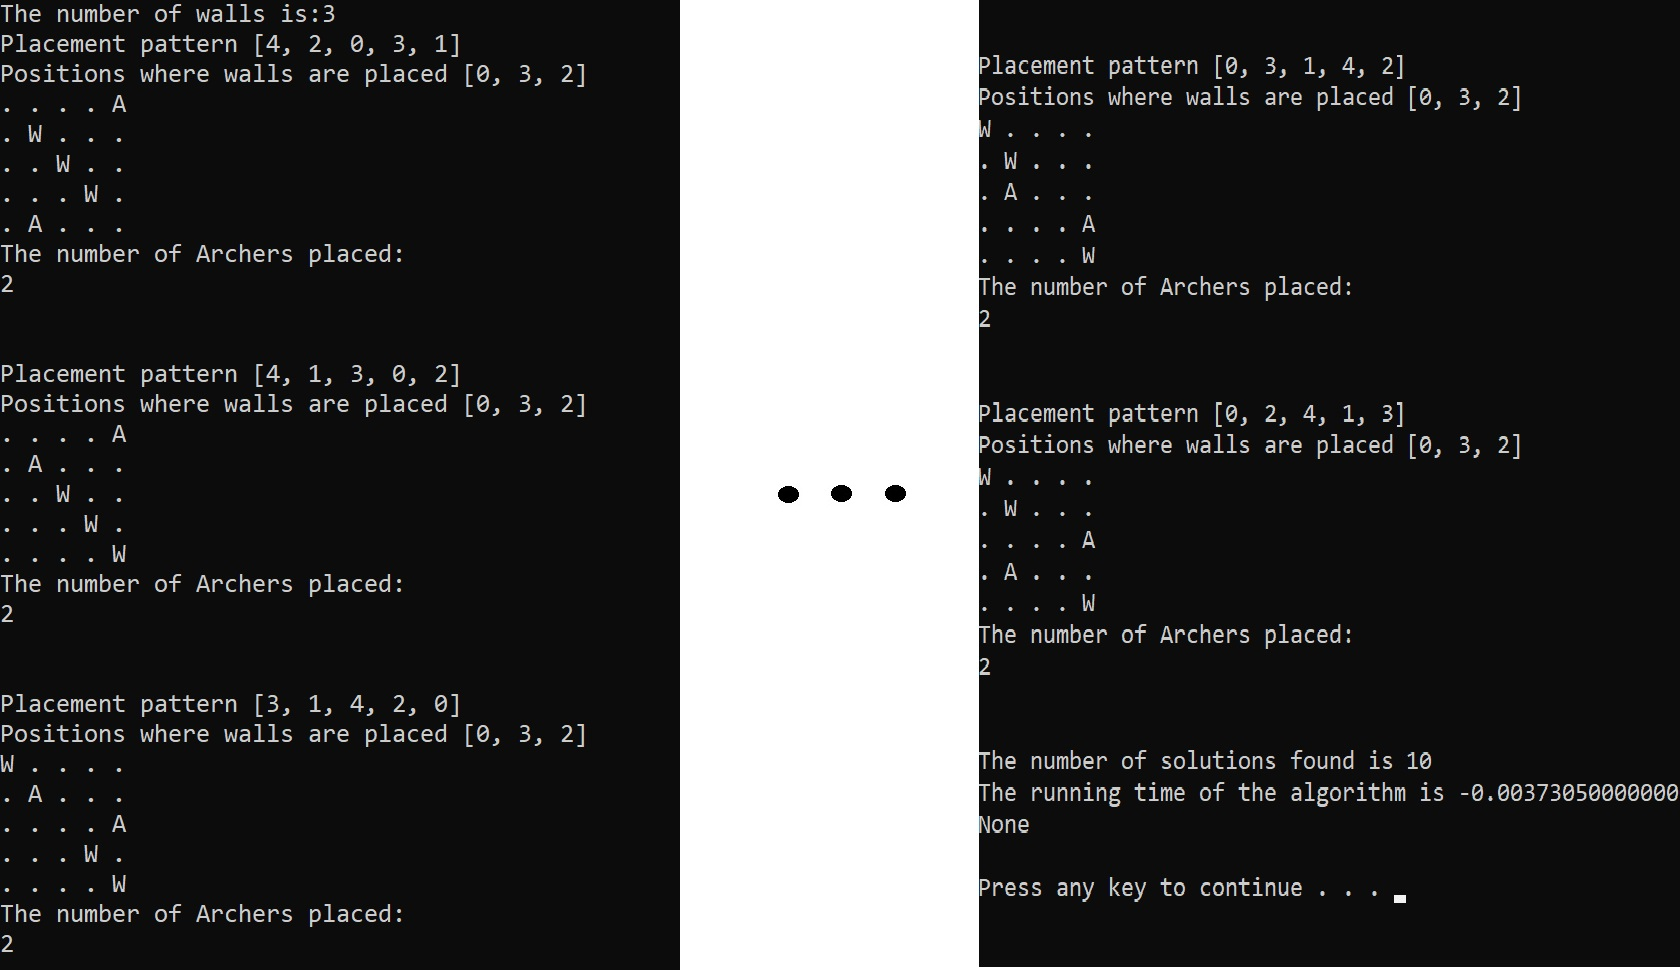
\includegraphics[width=12 cm, height=15cm]{test2}
\end{figure}
\newpage
\item third test(small test size,grid size:6,walls placed on positions:4,5,0,1)
\begin{figure}[h]
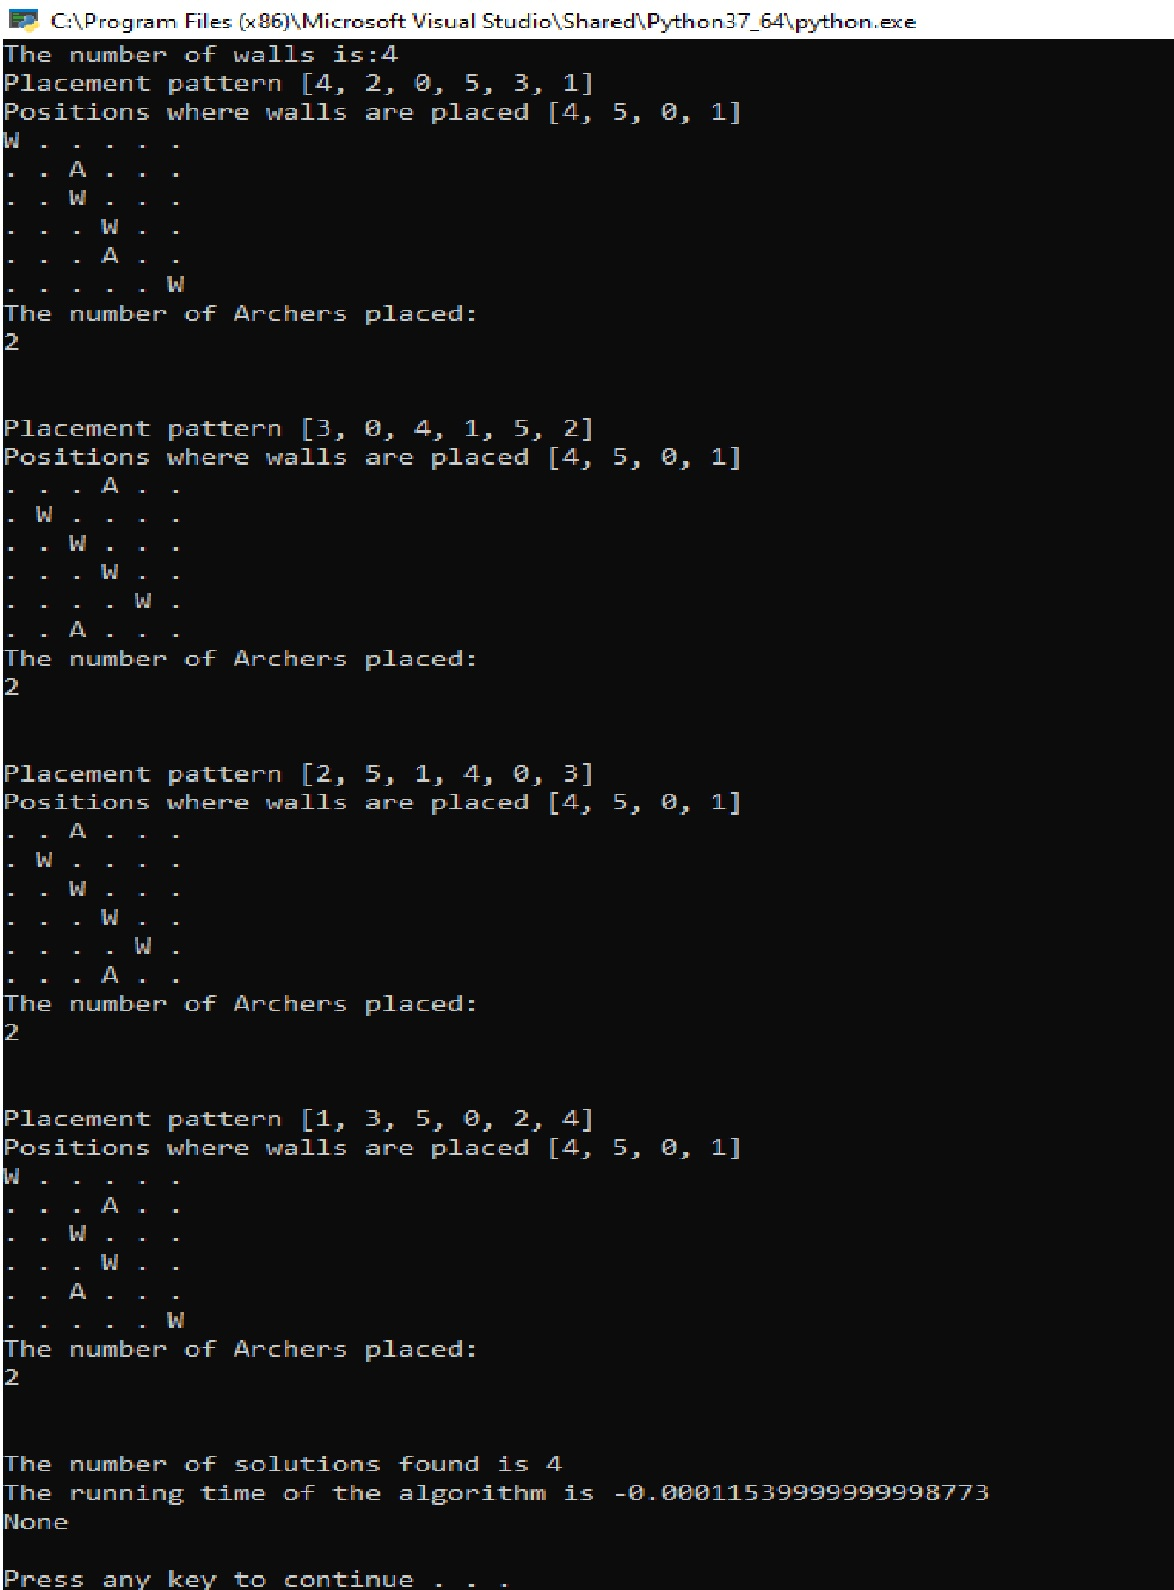
\includegraphics[width=12 cm, height=15cm]{test3}
\end{figure}

\newpage
\item fourth test(medium test size,grid size:7,walls placed on positions:1,3,2,4,max number of archers is 2(chaged the max to see how it affects the solutions))
\begin{figure}[h]
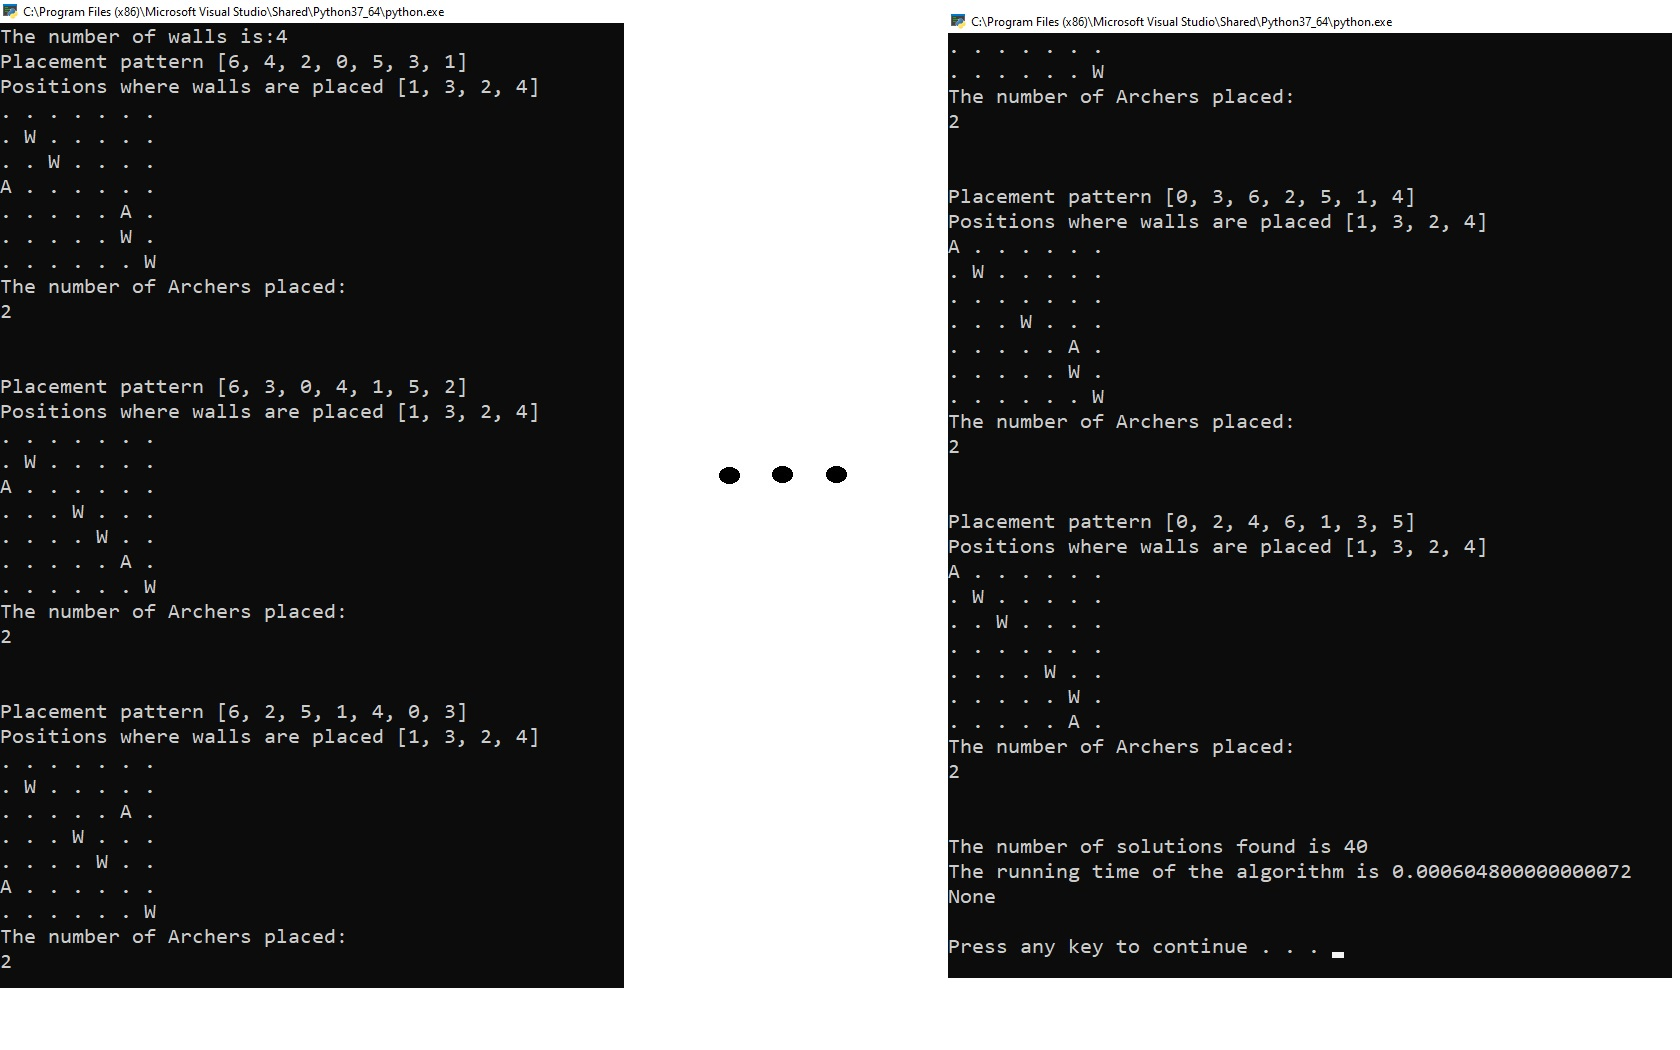
\includegraphics[width=12 cm, height=15cm]{test4}
\end{figure}

\newpage
\item fifth test(medium test size,grid size:8,walls placed on positions:3,1,,max number of archers is 4(chaged the max to see how it affects the solutions))
\begin{figure}[h]
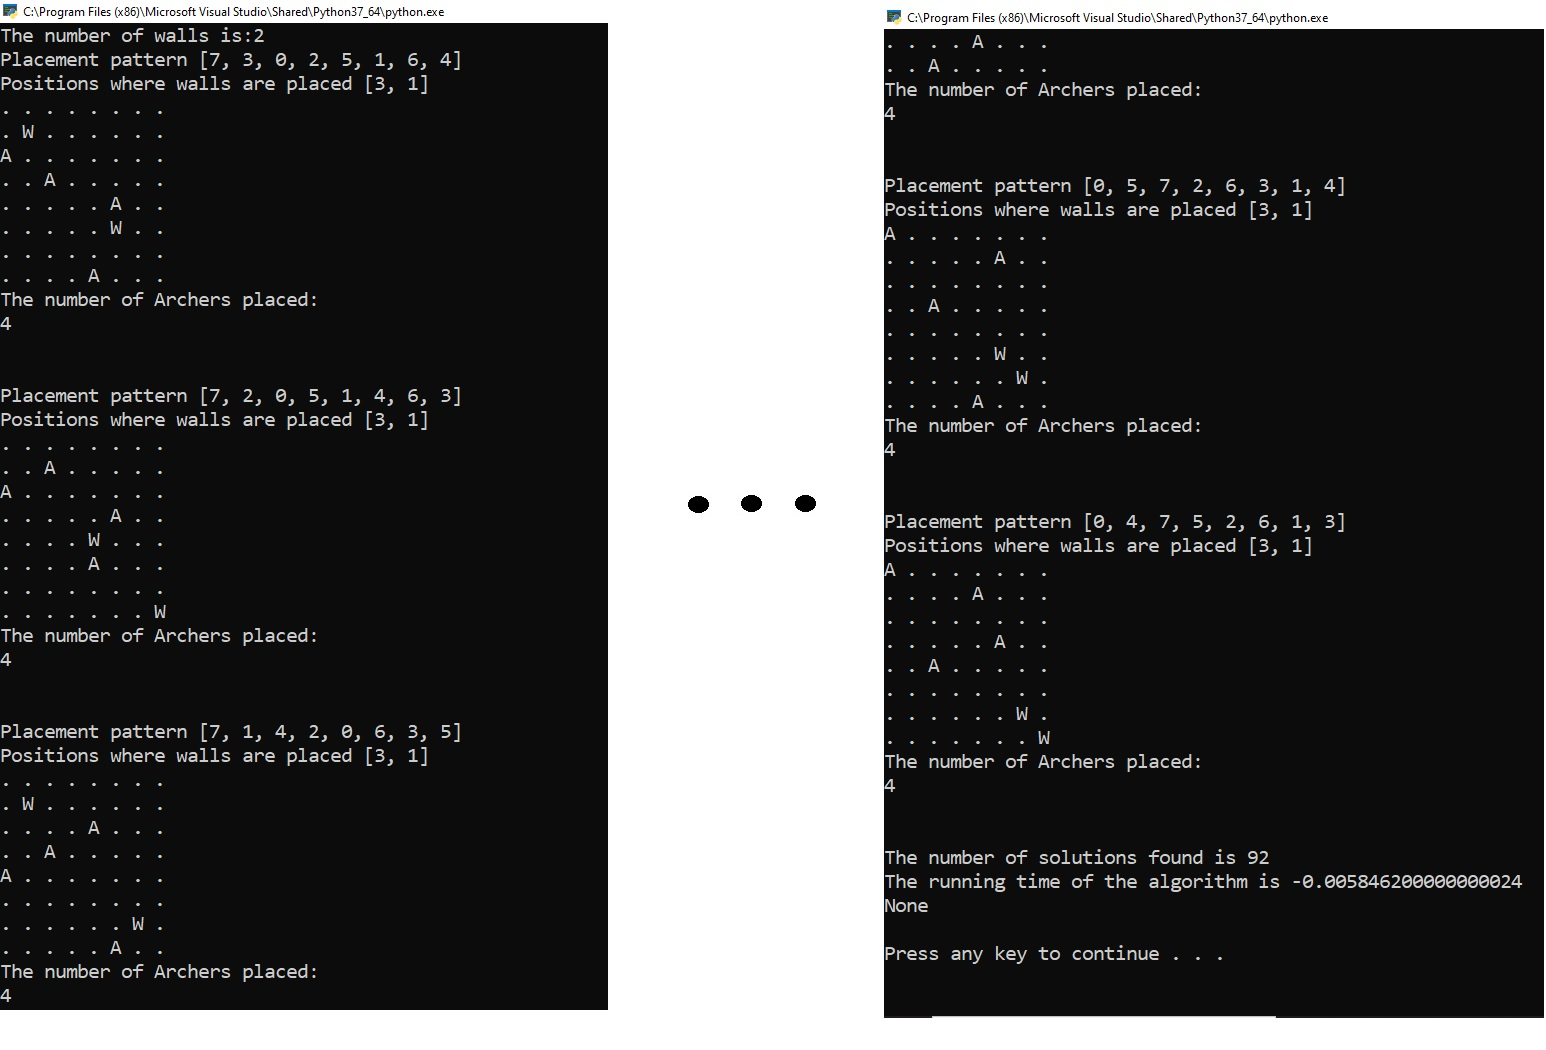
\includegraphics[width=12 cm, height=15cm]{test5}
\end{figure}


\newpage
\item sixth test(medium test size,grid size:9,walls placed on positions:6,3,1,from here I changed the maximum number of archers to match the size of the grid)
\begin{figure}[h]
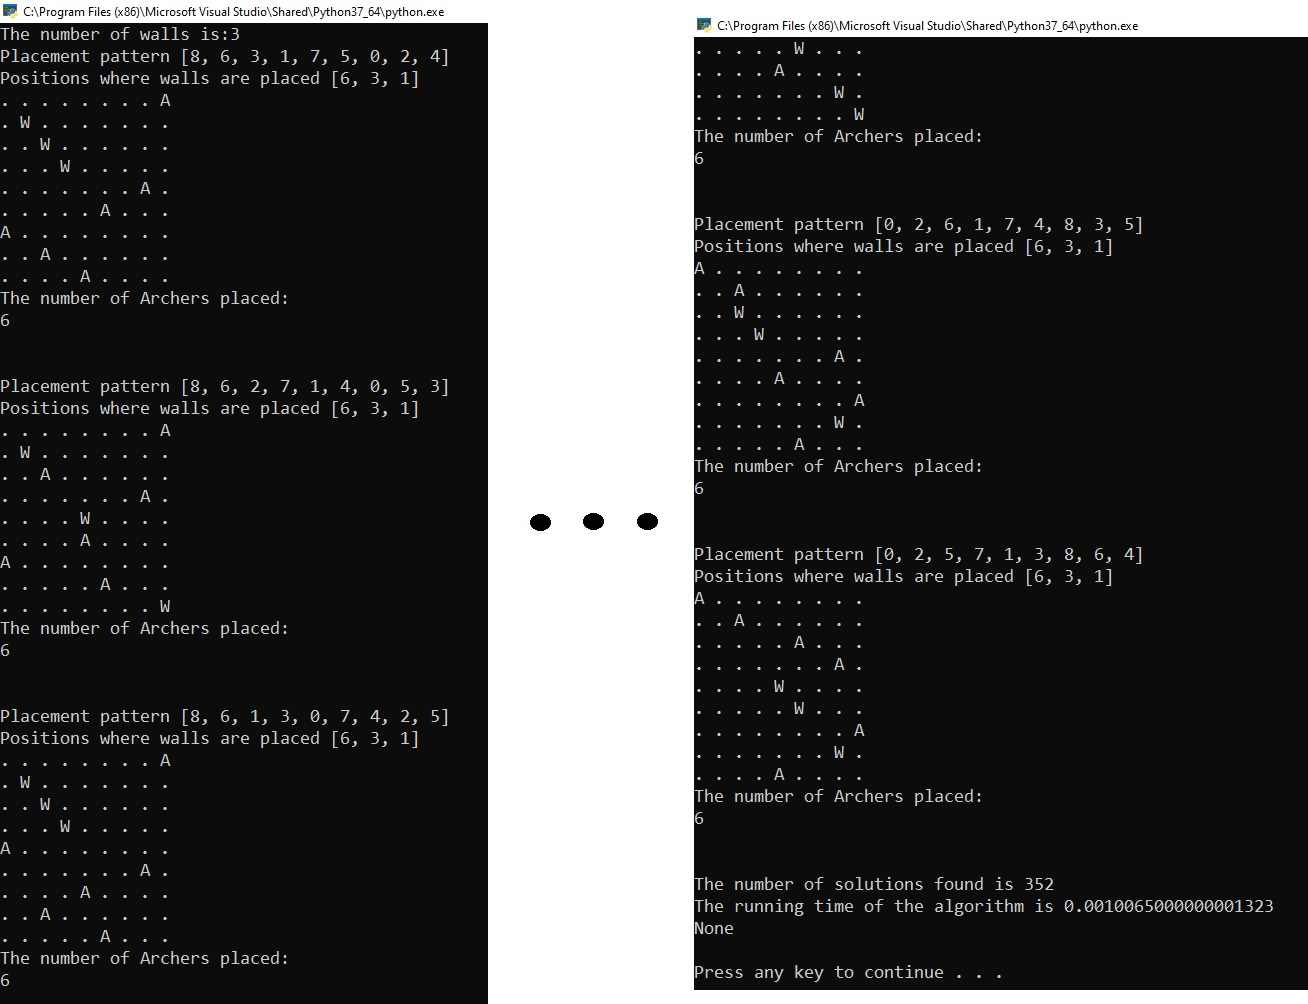
\includegraphics[width=12 cm, height=15cm]{test6}
\end{figure}

\newpage
\item seventh test(large test size,grid size:10,walls placed on positions:2,0,7,from here the running time begins to increase)
\begin{figure}[h]
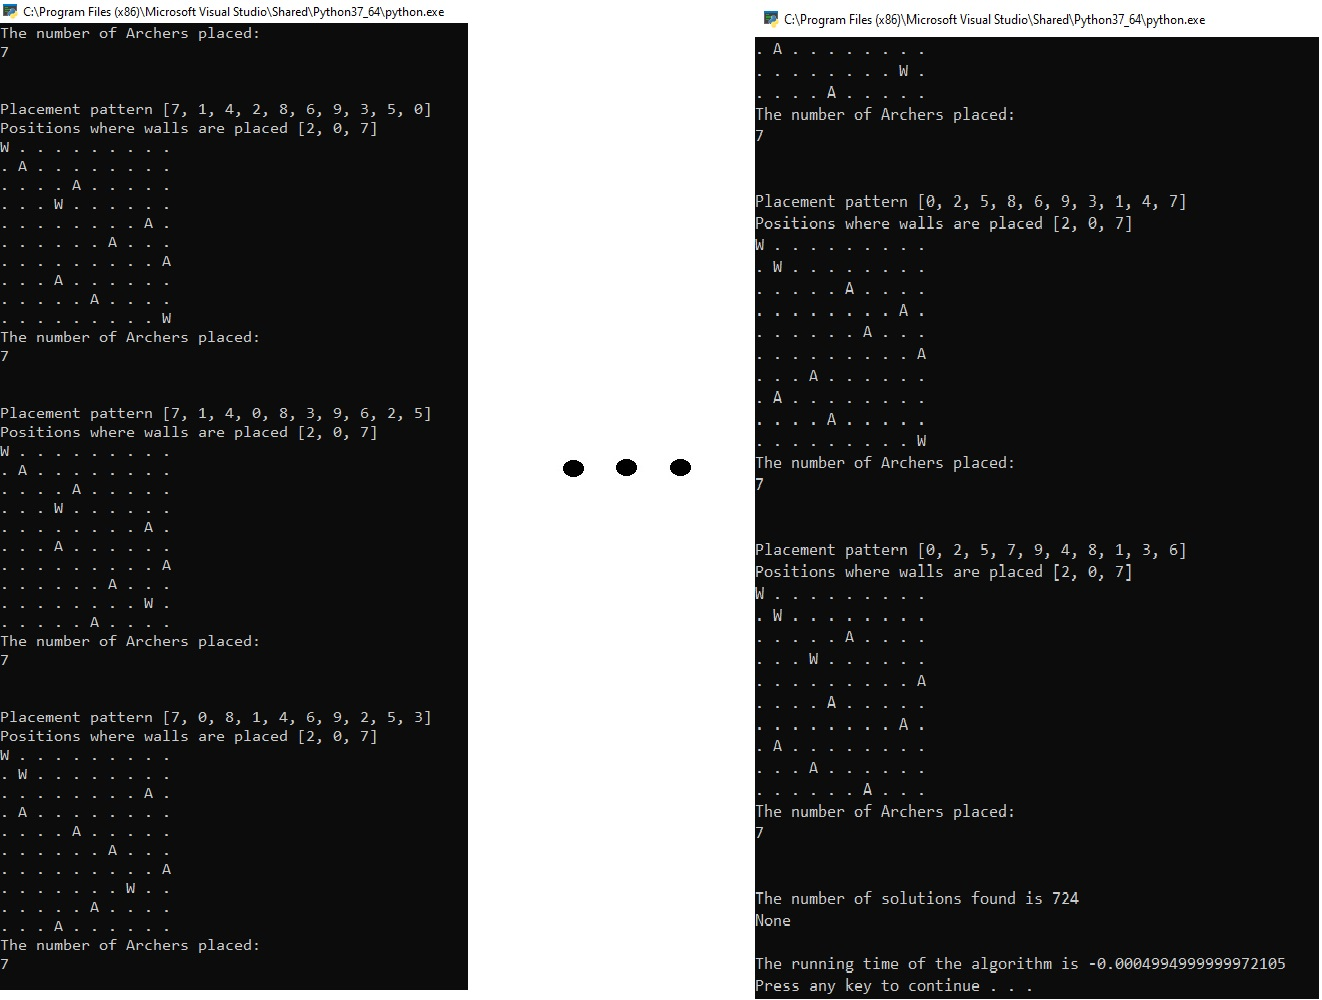
\includegraphics[width=12 cm, height=15cm]{test7}
\end{figure}

\newpage
\item eight test(large test size,grid size:10,walls placed on positions:0,8,4,1,9,6,7)
\begin{figure}[h]
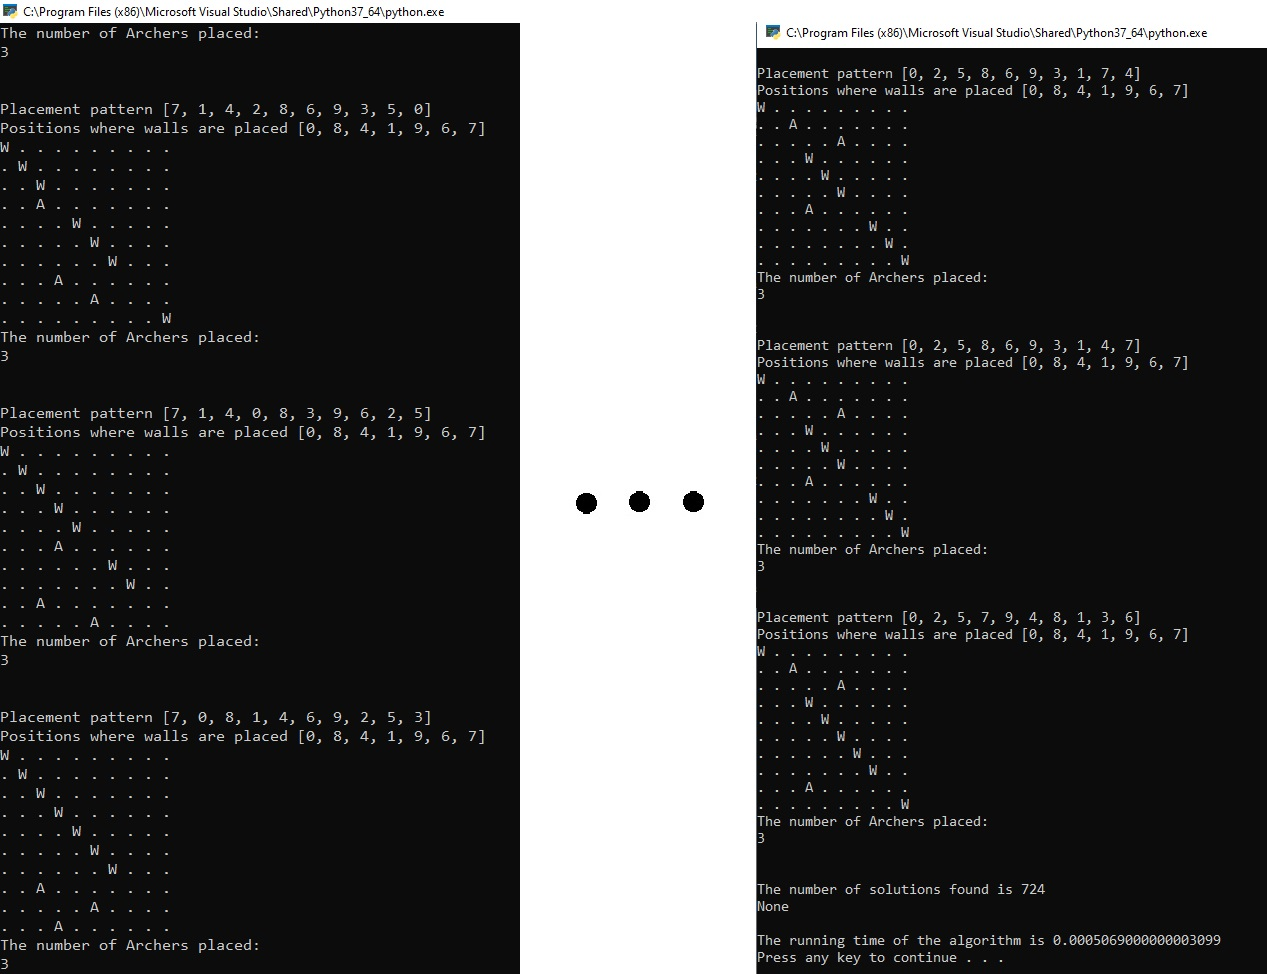
\includegraphics[width=12 cm, height=15cm]{test8}
\end{figure}

\newpage
\item ninth test(large test size,grid size:10,walls placed on positions:1)
\begin{figure}[h]
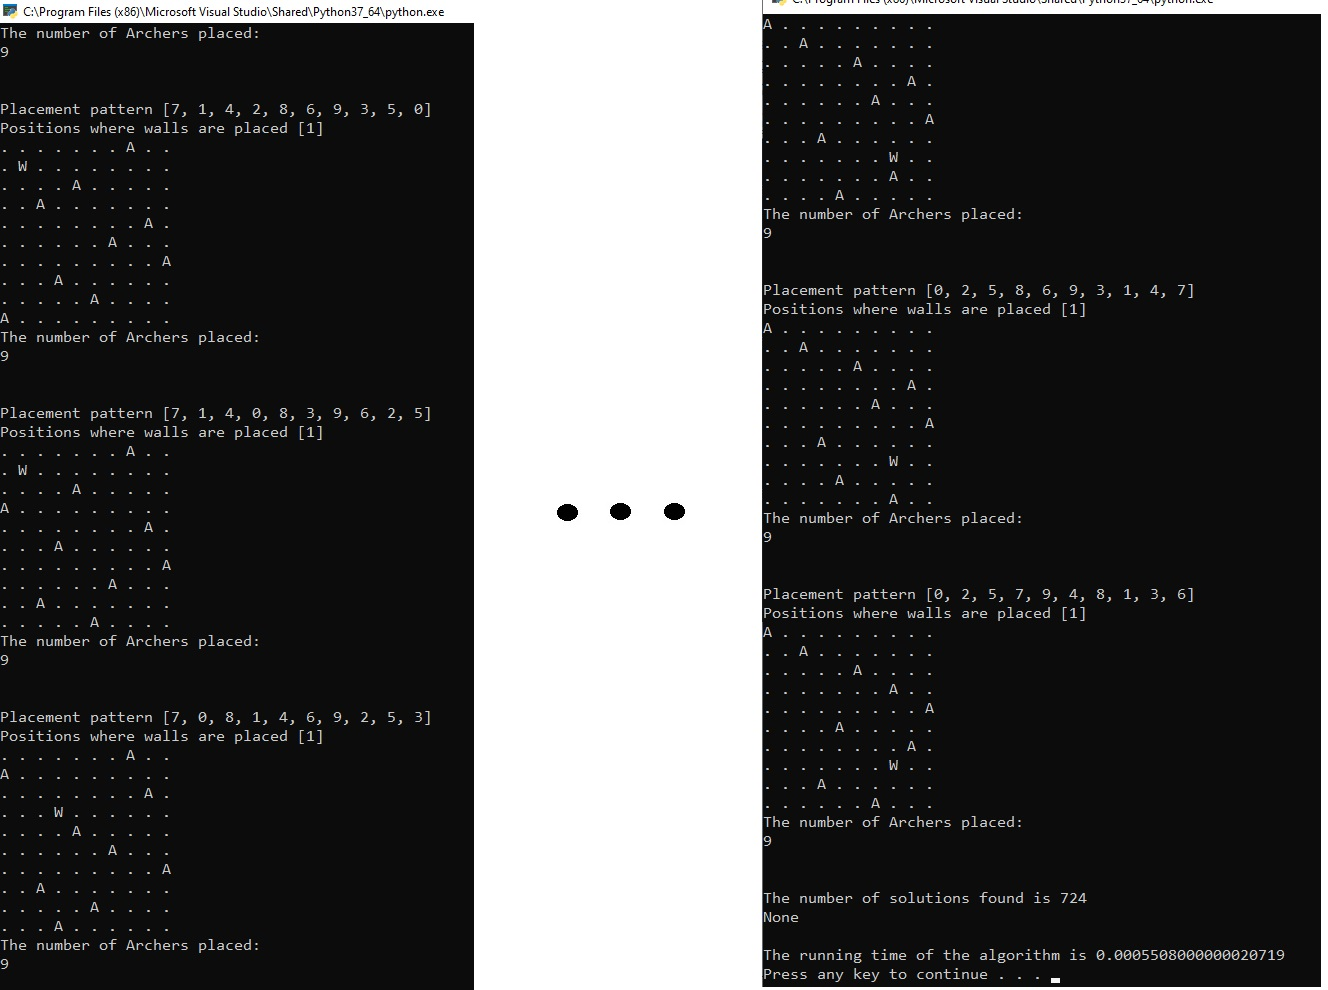
\includegraphics[width=12 cm, height=15cm]{test9}
\end{figure}

\newpage
\item tenth test(large test size,grid size:10,walls placed on positions:10,6,9)
\begin{figure}[h]
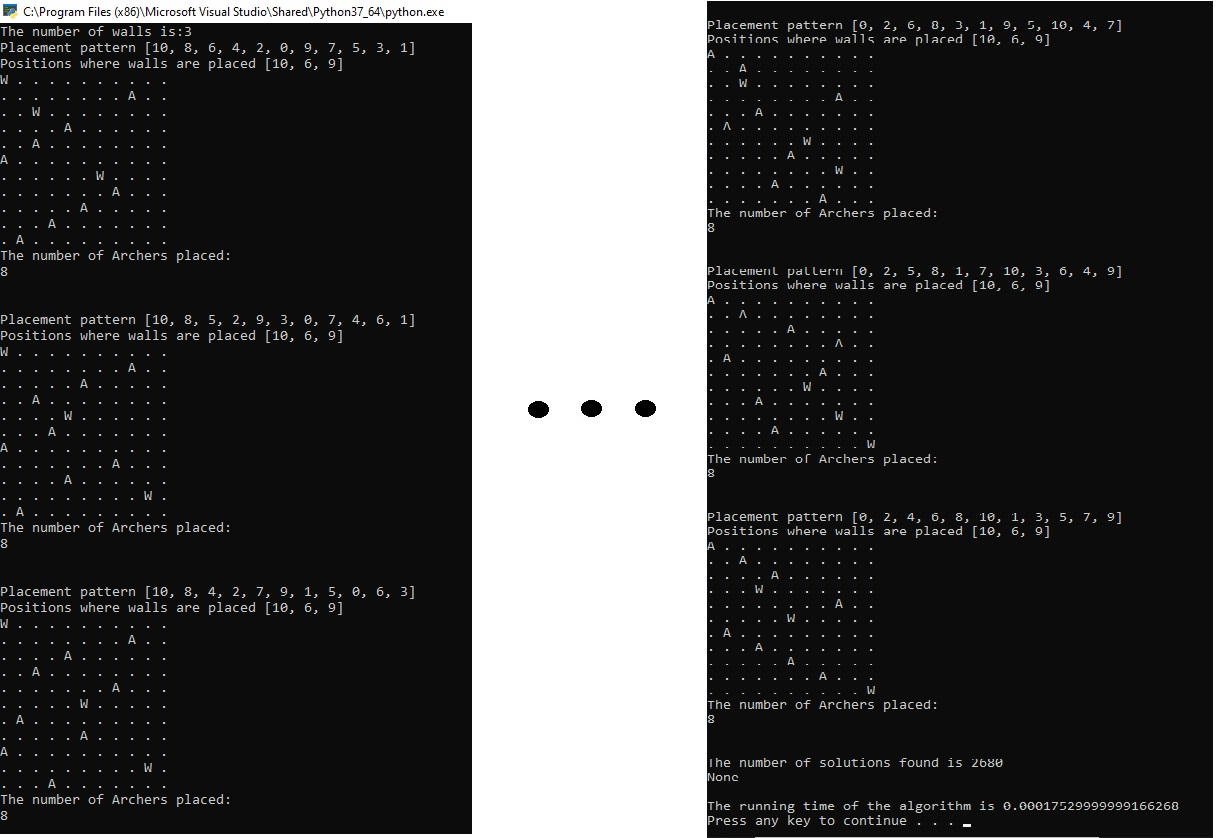
\includegraphics[width=12 cm, height=15cm]{test10}
\end{figure}

\end{enumerate}
\newpage
\section{Conclusions}
\LARGE
\par As we can see from the 10 tests that we made,the algorithm's data output is corresponding to how I implemented the problem.
\par We can observe that the solutions found and the running time of the algorithm(which you can  see in each picture at the bottom) get bigger the more we have a larger grid.
\par The output data sets design help us to both visualise the solution(by printing each grid with the Archers and Walls placed),but to also see the logic behind it,having displayed both the list which contains the positions of the archers as well as the position of the walls.
\end{document}


